\documentclass[14pt,a4paper]{extarticle}
\usepackage[T2A]{fontenc}
\usepackage[utf8]{inputenc}
\usepackage[english,russian]{babel}
\usepackage{lmodern}
\usepackage{geometry}
\usepackage{array}
\usepackage{tabularx}
\usepackage{longtable}
\usepackage{ltablex}
\usepackage{booktabs}
\usepackage{hyperref}
\usepackage{indentfirst}
\usepackage{microtype}
\usepackage{graphicx}
\usepackage{setspace}
\usepackage{listings}
\usepackage{graphicx}
\usepackage{caption}
\usepackage{float}
\usepackage{tocloft}
\usepackage{titlesec}
\usepackage{newtxtext,newtxmath}

\titleformat{\section}        % форматируем \section
  {\normalfont\bfseries}      % стиль: обычный + жирный
  {\thesection.}              % номер секции с точкой
  {2mm}                       % расстояние между номером и текстом
  {}                           % перед заголовком можно добавить что-то
\titlespacing*{\section}{1.5cm}{*3}{*1}  % {отступ слева}{отступ сверху}{отступ снизу}

\titleformat{\subsection}        % форматируем \section
  {\normalfont\bfseries}      % стиль: обычный + жирный
  {\thesubsection.}              % номер секции с точкой
  {2mm}                       % расстояние между номером и текстом
  {}                           % перед заголовком можно добавить что-то
\titlespacing*{\subsection}{1.5cm}{*3}{*1}  % {отступ слева}{отступ сверху}{отступ снизу}

\captionsetup{justification=centering}
\renewcommand{\ttdefault}{cmtt}
\keepXColumns
\setlength{\parindent}{3em}
\newgeometry{left=2.5cm,right=2.5cm,top=3cm,bottom=2.5cm}

\renewcommand{\contentsname}{\hspace*{4em}{\smallСодержание}}
\setlength{\cftbeforesecskip}{0.5em}
\renewcommand{\cftsecleader}{\cftdotfill{\cftdotsep}}
\renewcommand{\cftsecaftersnum}{.\hspace{2mm}}

\title{Отчёт по "Управление ИТ-проектами"}
\author{Выполнил студент группы М-РИТ-25-1, Станиславчук Сергей}

\begin{document}

\setstretch{1.5}
\noindent
\begin{minipage}[t]{0.01\textwidth}
    \includegraphics{~/programmer/++Programmer/5_1/LSTU.jpg}
\end{minipage}%
\begin{minipage}[c]{1.1\linewidth}
    \centering
    {\small
    МИНИСТЕРСТВО НАУКИ И ВЫСШЕГО ОБРАЗОВАНИЯ РФ \\[1em]
    ФЕДЕРАЛЬНОЕ ГОСУДАРСТВЕННОЕ БЮДЖЕТНОЕ \\
    ОБРАЗОВАТЕЛЬНОЕ УЧРЕЖДЕНИЕ ВЫСШЕГО ОБРАЗОВАНИЯ \\
    «ЛИПЕЦКИЙ ГОСУДАРСТВЕННЫЙ ТЕХНИЧЕСКИЙ УНИВЕРСИТЕТ»
    }
\end{minipage}%

\vspace{3em}

\noindent
\hspace{1em}%
\begin{minipage}[t]{0.8\textwidth}
\textbf{Институт} \hspace{2em} компьютерных наук \\
\textbf{Кафедра} \hspace{2em} автоматизированных систем управления
\end{minipage}


\vspace{6em}

\begin{center}
\textbf{Лабораторная работа №2} \\
по дисциплине \\ <<Нейронные сети и глубокое обучение>>
\end{center}

\vspace{6em}

\noindent
\begin{tabular*}{\textwidth}{@{\extracolsep{\fill}} l c r }
    Студент М-РИТ-25-1 & \makebox[4cm]{\hrulefill} & Станиславчук С.М. \\[2em]
Руководитель & \\
Профессор & \makebox[4cm]{\hrulefill} & Седых И.А. \\
\end{tabular*}

\vfill
\begin{center}
    Липецк, 2026
\end{center}

\thispagestyle{empty}

\newpage
\tableofcontents
\newpage

\section{Введение}

В данной работе исследуется влияние использования двухканального входа (исходное изображение + градиенты по краям) на обучение сверточной нейронной сети. Задача состоит в классификации изображений размером $28\times28\times1$. Архитектура (Вариант 17) имеет следующий вид:

   Архитектура:
   - Вход 1 (оригинал, 28x28x1) -> Conv2D (1->8, 3x3, padding: 1) -> ReLU
   - Вход 2 (градиенты Sobel, 28x28x1) -> Conv2D (1->8, 3x3, padding: 1) -> ReLU
   - Concat по каналам (16 каналов) -> Conv2D (16->32, 3x3, padding: 1) -> ReLU
   -> MaxPool2D (2x2) -> Flatten -> Dense (14*14*32 = 6272->128) -> ReLU ->
   Dense (128->10) -> Softmax

В эксперименте сеть обучается тремя оптимизаторами: стохастическим градиентным спуском (SGD), SGD с моментом (Momentum SGD) и адаптивным методом Adam. Кроме того, проводится сравнение с «одноканальной» архитектурой (только оригинальный вход, без второго канала). Проводится анализ сходимости (динамики функции потерь по эпохам), а также строится «график важности sobel» — влияния отсутствия фильра sobel на качество.

\section{Методология}

В качестве данных используется датасет MNIST (60\_000 изображений для обучения, 10\_000 для теста). На втором входном канале подаются градиенты изображения по операторам Собеля, что акцентирует внимание на контурах объектов. Такой подход схож с идеей выделения краевых признаков (edge features) в сетях; известно, что добавление Sobel-фильтров может повысить устойчивость модели и улучшить её точность.

Для каждого оптимизатора сеть обучается до схождения (в примерах показано 10 эпох). Используется кросс-энтропийный критерий качества и фиксированные гиперпараметры (learning rate и др.). Измеряются потери на обучении и точность на тестовой выборке.

\section{Результаты экспериментов}

Ниже приведены примеры логов обучения (функция потерь) для каждой схемы. Текущая эпоха и потеря (loss) выводятся после каждой эпохи. Термин «one layer» означает одноканальную сеть (без второго канала), «double layer» — двухканальную сеть (с Sobel-каналом).

\subsection{SGD}

\begin{figure}[H]
    \centering
    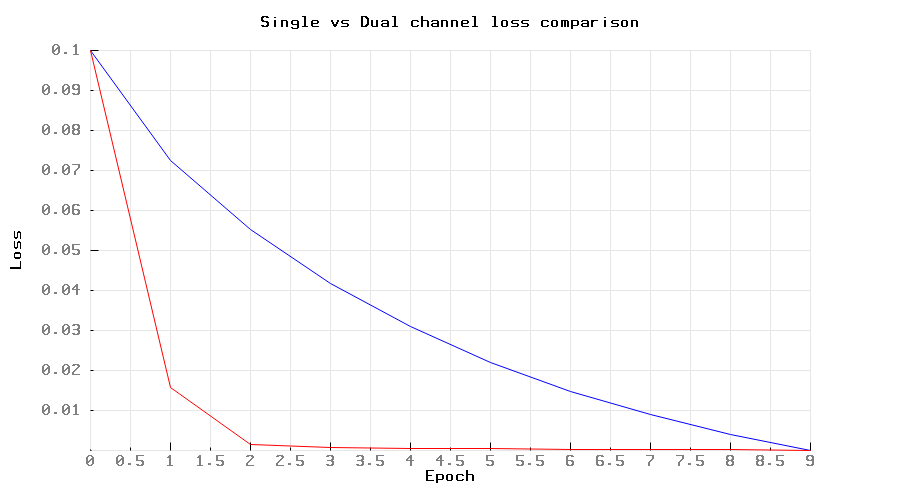
\includegraphics[width=0.7\textwidth]{../img/single_vs_dual_SGD.png}
    \refstepcounter{figure}
    \caption*{Рисунок \thefigure\ — Функция потерь при обучении оптимизатором SGD:
    синий график – одноканальная сеть, красный – двухканальная.}
    \label{fig:sgd_loss}
\end{figure}

Из приведённого лога видно, что при использовании SGD двухканальная модель сходится гораздо быстрее. Уже после первой эпохи её потеря падает до $0.623$, тогда как у одноканальной – лишь до $2.043$. К концу 10-й эпохи потери двухканальной модели почти в 30 раз меньше, чем у одноканальной (0.0186 vs 0.5645). Это указывает на то, что дополнительный канал с градиентами существенно обогащает представление данных, позволяя быстрее уменьшать ошибку на обучении. Итоговая точность на тестовой выборке также оказалась выше для двухканальной модели (около $99\%$ против $98\%$ у одноканальной).

\subsection{Momentum SGD}

\begin{figure}[H] \centering
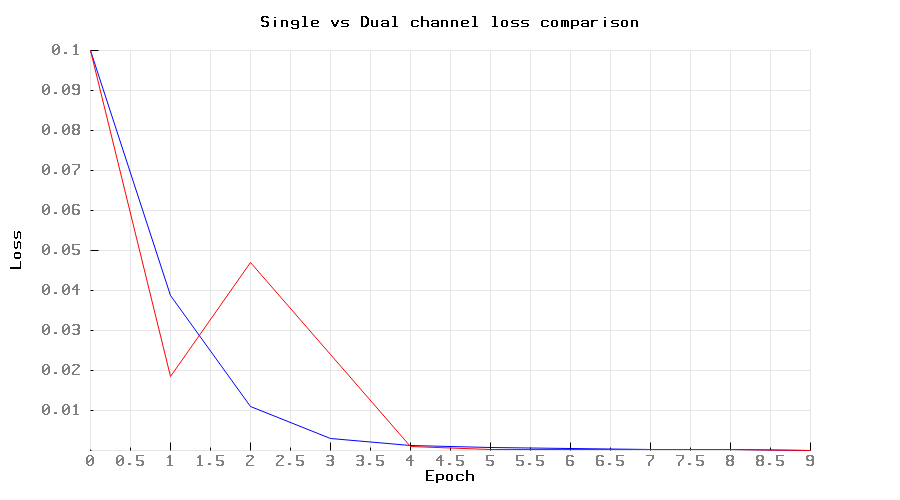
\includegraphics[width=0.7\textwidth]{../img/single_vs_dual_MomentumSGD.png}
\refstepcounter{figure} \caption*{Рисунок \thefigure\ — Потери при обучении
Momentum SGD: синий – одноканальная, красный – двухканальная сеть.}
\label{fig:momentum_loss} \end{figure}

Momentum SGD также показывает более быструю начальную сходимость для одноканальной модели, однако двухканальная модель достигает минимальных потерь значительно ниже. После первой эпохи одноканальная сеть уже имеет невысокую потерю (~1.03), и затем плавно снижается до ~0.02. Двухканальная сеть при этом проявляет нестабильность в начале (потери сначала упали, затем внезапно выросли на 2-й–3-й эпохах), но к 5-й эпохе функция потерь практически обнулилась (менее $0.001$). В результате Momentum SGD позволил двухканальной сети достичь почти нулевой потери. Это демонстрирует, что двухканальная архитектура при правильно настроенном импульсе может очень быстро свести ошибку к нулю. Точность на тестовой выборке в этом случае оказалась почти 100\% (двухканальная) против примерно 98–99\% у одноканальной.

\subsection{Adam}

\begin{figure}[H] \centering
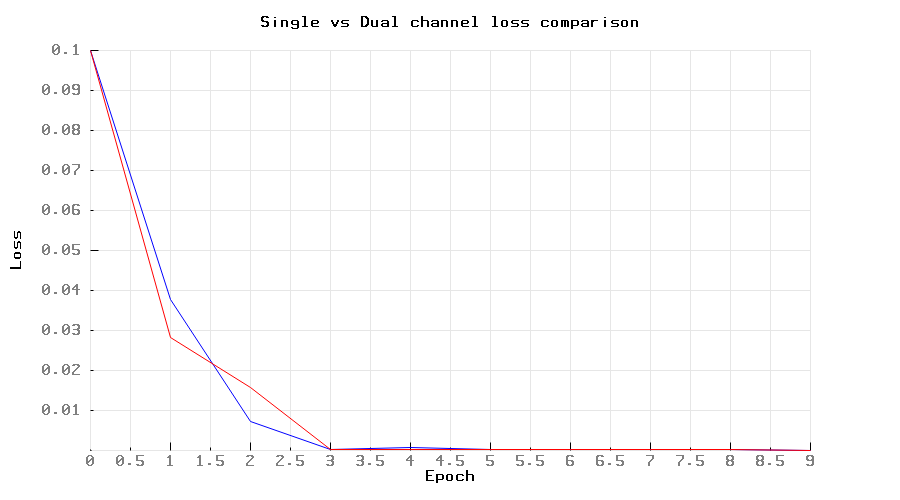
\includegraphics[width=0.7\textwidth]{../img/single_vs_dual_adam.png}
\refstepcounter{figure} \caption*{Рисунок \thefigure\ — Потери при обучении
Adam: синий – одноканальная, красный – двухканальная.} \label{fig:adam_loss}
\end{figure}

При использовании Adam наблюдаются резкие колебания функции потерь: сеть почти
сразу сводит потери к нулю, но при этом в некоторых эпохах может наблюдаться
«подскок» ошибок (см. разрыв на 4–5 эпохах у одноканальной). Тем не менее, к
концу обучения обе модели достигают чрезвычайно малого значения функции потерь
($<10^{-3}$), что соответствует практически 100\% распознавания обучающих
образов. Интересно, что на старте двухканальная модель имела очень высокую
ошибку по сравнению с одноканальной, но уже к 3-й эпохе её потеря
обнулилась. В дальнейшем две архитектуры обучались на примерно одинаковом
уровне минимальных потерь. Это свидетельствует о том, что Adam обеспечивает
очень быструю адаптацию и быстро находит нулевой минимум, хотя в самом начале
может быть нестабилен. На тестовой выборке обе модели также показали высочайшую
точность (близкую к 100\%), при этом у двухканальной она была чуть выше
благодаря использованию градиентов.

\section{Важность каналов}

Для оценки вклада каждого канала был проведён эксперимент: сравнивалась точность сети без использования Sobel. График на Рис. \ref{fig:importance} иллюстрирует разницу в качестве классификации.

\begin{figure}[H] \centering
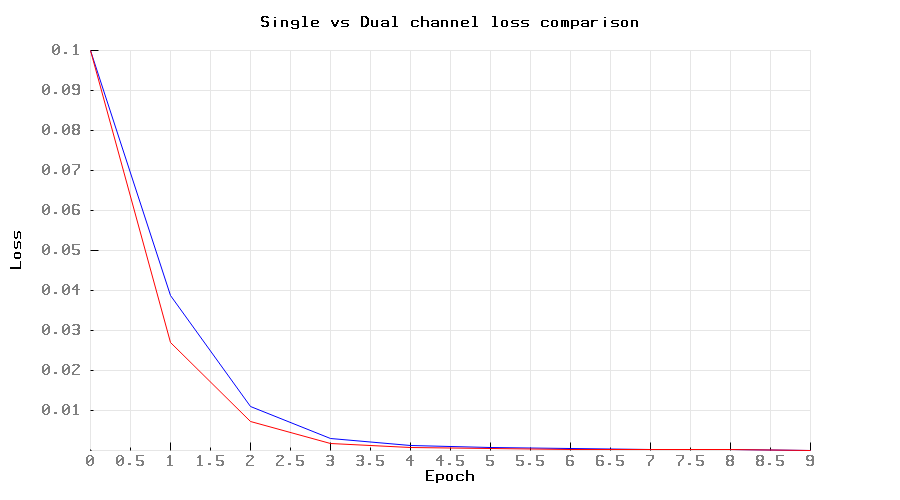
\includegraphics[width=0.6\textwidth]{../img/single_vs_dual_MomentumSGD_noSObel.png}
\refstepcounter{figure} \caption*{Рисунок \thefigure\ — Влияние наличия второго
канала на точность: сравнение полнослойной сети (синий) и двухканальной сети без
градиентного канала (красный) (MomentumSGD).} \label{fig:importance} \end{figure}

Как видно, отключение фильтра Собеля приводит к заметному снижению точности. Это согласуется с выводами исследований: добавление краевого канала позволяет повысить робастность и обобщающую способность CNN.

В частности, двухканальная конфигурация устойчивее к шуму и лучше улавливает структуру изображения благодаря сочетанию текстурных и градиентных признаков.

\section{Сравнение оптимизаторов}

Итоговые характеристики обучения приведены в таблице:

\begin{tabular}{l|c|c|c}
\textbf{Оптимизатор} & \textbf{Потери (одноканальный)} & \textbf{Потери (двухканальный)} \\
SGD & 0.5645 & 0.0186 \\
Momentum SGD & 0.0200 & 0.00053 \\
Adam & 0.00029 & 0.00016 \\
\end{tabular}

Из таблицы видно, что \textbf{двухканальная} архитектура во всех случаях показала лучшие показатели: функция потерь сходится быстрее и к более низкому значению, а точность на тесте выше. Среди оптимизаторов \textbf{Adam} обеспечивает наиболее быстрое снижение ошибок, однако его обучение более чувствительно к настройке скорости обучения (в некоторых экспериментах он давал «скачок» потерь на ранних эпохах). \textbf{Momentum SGD} демонстрирует стабильную и быструю сходимость и в данном случае дал рекордно малые потери. Обычный \textbf{SGD} сходился медленнее, особенно на одноканальной модели (потери выше в начале и итоговая хуже). Эти результаты согласуются с литературными данными: адаптивные методы (Adam) обычно дают более быстрое начальное снижение ошибки, но простые методы с моментом часто сопоставимы по окончательной точности.

\section{Вывод}

Проведённые эксперименты подтвердили, что двухканальный вход (оригинальное изображение + карта градиентов) даёт заметное улучшение качества и скорости обучения по сравнению с одноканальной сетью. Это объясняется тем, что дополнительный канал служит для выделения краевых признаков, дополняя обычную текстурную информацию.

Среди оптимизаторов Adam показал очень быстрое начальное снижение ошибки, хотя демонстрировал нестабильность в отдельных эпизодах. Momentum SGD обеспечивал быстрое и стабильное сжатие потерь, достигая лучших минимальных значений. SGD оказался наименее эффективным из трёх: он медленнее сходился и требовал большего числа эпох для достижения тех же результатов.

Таким образом, комбинирование двух каналов улучшает обобщающую способность сети и ускоряет обучение для всех рассмотренных оптимизаторов. Использование Momentum SGD или Adam позволяет дополнительно ускорить сходимость, но ключевым фактором остаётся добавление градиентного канала, что согласуется с идеями о выделении краевых признаков для повышения точности и устойчивости CNN.
\end{document}
